\documentclass[a4paper,10pt]{article}
\usepackage[utf8]{inputenc}
\usepackage[english] {babel}
\usepackage[T1]{fontenc}
\usepackage{lmodern}
\usepackage{graphicx}
\usepackage{graphics}
\usepackage{ulem}
\usepackage{amssymb}
\usepackage{url}
\usepackage{circuitikz}
\usepackage{subfig}
\usepackage[a4paper]{geometry}
\geometry{hscale=0.7,vscale=0.7,centering}
\usepackage{vmargin}
\usepackage{amsmath}
\usepackage{amssymb}
\usepackage{amsthm}
\usepackage{moreverb}
\usepackage{listings}
\usepackage{qtree}
\graphicspath{{IMAGES/}}
\newtheorem{theorem}{Théorème}[section]
\newtheorem{defi}{Définition}[section]
\newtheorem{propri}{Propriété}[section]
\newtheorem{ex}{Exemple}[section]
\newtheorem{thesis}{Thèse}[section]
\newtheorem{cor}{Corollaire}[section]

\usepackage{color}

\definecolor{gris}{rgb}{0.95,0.95,0.95}


% Param�rage des listings
\lstset{basicstyle=\footnotesize\ttfamily}
\lstset{keywordstyle=\color[rgb]{0,0,1}\bfseries}
\lstset{identifierstyle=\color{black}}
\lstset{commentstyle=\color[rgb]{0,0.4,0}}
\lstset{stringstyle=\color[rgb]{0.7,0,0}}
\lstset{showstringspaces=false}
\lstset{showtabs=false}
\lstset{tabsize=3}
\lstset{extendedchars=true}
\lstset{breaklines=true}
\lstset{postbreak={}}
\lstset{breakautoindent=true}
\lstset{breakindent=0pt}
\lstset{xleftmargin=0.1cm}
\lstset{xrightmargin=0cm}
\lstset{frame=tb,rulecolor=\color[gray]{.4}}
\lstset{captionpos=b}
\lstset{aboveskip=0.5cm,belowskip=0.5cm}
\lstset{numbers=left}
\lstset{columns=fixed}
\lstset{language=java}



\newcommand{\code}[1]{\lstinline{#1}}

\setlength{\parskip}{.7em}

\begin{document}


\begin{flushleft}

\includegraphics[scale=0.3]{logo_ist.jpeg}
\end{flushleft}


\vspace{1cm}

\begin{center}{
\scshape{\LARGE Wolves and squirrel : Part 1 }}

\vspace{0.5cm}
\hbox{\raisebox{0.4em}{\vrule depth 0pt height 0.05cm width 16cm}}
{\setlength{\parskip}{0.2cm}

 \Huge
 \bfseries
 \LARGE  Parallel and Distributed Computing
 \\
CPD \\

\vspace{0.2cm}

}
\vspace{0.5cm}

\hbox{\raisebox{0.4em}{\vrule depth 0pt height 0.05cm width 16cm}}
\vspace{2.5cm}


\end{center}

\vspace{3cm}


\vfill
\begin{flushright}
\textbf{Group 30 :}\\
Cappart Quentin (77827)\\
Mikołaj Jakubowski (77610)\\
Paulo Tome (72419)\\

\end{flushright}
\newpage

\setcounter{page}{1}

\renewcommand\thepage{\arabic{page}}


\newpage

\section*{Decomposition done}

To understand our decomposition, we must explain before how our serial version works.
The main work are done in the huge worldLoop :

\begin{lstlisting}
for(i = 0 ; i < 4 * noOfGenerations ; i++){...}
\end{lstlisting}

What is particular is that we iterate to 4 times the number of generations. This structure was done to do the following things :

\begin{enumerate}
 \item We proceed the red generation and we keep all the conflicting movement.
 \item We deal with the conflicting movement of the red generation.
 \item We proceed the black generation and we keep all the conflicting movement.
 \item We deal with the conflicting movement of the black generation.
\end{enumerate}

Each part are done in one particular iteration, the correct action are chosen thanks to modulo and conditional operation.
With this structure we don't want to parallelize this main loop, but only his content. 
And after each iteration we need to synchronize. So, our parallelization are done like this 

\begin{lstlisting}
#pragma omp parallel for private(x,y,cell)
for(y = 0 ; y < worldSideLen ; y++){
      for(x = 0 ; x < worldSideLen ; x++){
	      //proceeding the cells
      }
)
\end{lstlisting}

Let's notice that we only parallelize on the row and not on the column because of the cache and to keep the adjacent portion of memory
together.

\section*{Conflict resolution}

The conflict resolution is done by the architecture of the serial version. Indeed, all the conflicting movement are not made
directly but their are kept in memory and proceeded after each subgeneration with the \texttt{update} method.
So, with the parallelization, given that we have an implicit synchronization after each iteration of the main loop (generation loop),
the conflict are implicitly resolved. We made sure after that our outputs with severals threads are always the same than the serial version.

\section*{Load Balancing}
Logic of every sub-generation is divied in two steps. 
Selecting updates and updating itself. 
Second phase is done per cell, so it is easy to parallelize. 
Every cell has a list of updates that needs to be invoked on it. 
Load balancing is done by diving those lists evenly between cores by dynamic sheduling. It's done by this pragma
in the \texttt{update} fonction :

\begin{lstlisting}
 #pragma omp parallel for schedule(dynamic,1)
\end{lstlisting}

We add it in the code, but it gave a slower execution time, so we didn't integrate it in our final version.

\section*{Performances analyze}

The following array recaps the execution time of the OMP version with severals numbers of threads.
\begin{table}[!ht]
\centering
\begin{tabular}{|r||r|r|r|r|}
  \hline
    Instance     & 1 thread   & 2 threads   & 4 threads  & 8 threads  \\
  \hline
    ex3.in       &  0.008     & 0.008        & 0.017       &  0.020 \\ 
  \hline
    world\_10.in &  0.011      &  0.006       & 0.021       & 0.035 \\ 
  \hline
   world\_100.in &  0.111      & 0.070        & 0.068      & 0.1278 \\ 
  \hline
  world\_1000.in &  12.885   & 7.712       & 6.534      &  6.522 \\ 
  \hline
\end{tabular}
\caption{Performances (in sec) for the different instances.}
\end{table}

We did these experiments on a computer with 4 cores with the input \texttt{instance 10 9 8 100}. We
let to the "iteration print" in the code\footnote{If we remove it, the execution time is to fast to do an useful analyze.}.
First, we notice that for the smallest instance, \texttt{ex3.in},
more threads we have, the program is slower. This was expected. Indeed, given that the instance are small, the overhead of the threads (creation, repartition and
synchronization for example), surpass the gain of multithreading.
For the instance \texttt{world\_10.in}, we notice it from 4 threads.
For the biggest instance, \texttt{world\_1000.in}, we see the speedup when we deal with severals threads. The speedup per core decreases with the number
of threads\footnote{We gain more from 1 to 2 threads than for 2 to 4 threads.}.
Finally, given that the computer has 4 cores, we are not interested in creating more than.
\\

Now, let's compare the execution time for  world\_1000.in with the ideal speedup\footnote{$S = \frac{T_{serial}}{N_{threads}}$}
with different numbers of threads :

\begin{figure}[!ht]
  \centering
  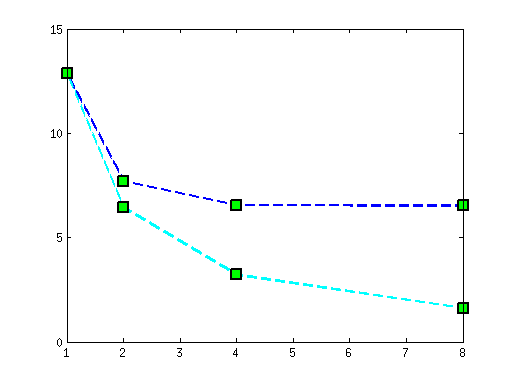
\includegraphics[width=8cm]{speedup.png}
  \caption{Comparison with the ideal speedup.}
\end{figure} 

With two threads we are relatively close to the ideal speedup. However the gap grows with more threads. We expected this king of results.
Indeed, there is always overhead when we deal with threads and not all of our code is multithreaded, so it's normal that we don't reach
the ideal result.
\end{document}

